This section uses ANSYS Mechanical FEA software \cite{ANSYS} to validate analytical findings from previous sections. Please note that all results presented in the foregoing section utilizes USC units however, important results will be converted to their respective SI units. The overall ANSYS geometry is first presented followed by a series of FEA runs which are summarized below (see Table~\ref{table:4_runs}).

\begin{table}[H]
  \centering
  \caption{Labeling of FEA runs.}
    \begin{tabular}{cll}
    \textbf{Run} & \textbf{Focus} & \textbf{Description}\\
    \hline
    1A    & Drum Stress & Fixed ends, uniform $p$\\
    1B    & Drum Stress & Simply supported ends, uniform $p$ \\
    2A    & Drum Stress & Fixed ends, Capstan $p, z=24.5$, various $\mu$ \\
    2B    & Drum Stress & Simply supported ends, Capstan $p, z=24.5$, various $\mu$ \\
    2C    & Drum Stress & Fixed ends, Capstan $p, z=0$, various $\mu$ \\
    2D    & Drum Stress & Simply supported ends, Capstan $p, z=0$, various $\mu$ \\
    3     & Drum Buckling & Simply supported ends, uniform $p$ \\
    4     & Flange Stress & Fixed ends, uniform $p$ \\
    \end{tabular}%
  \label{table:4_runs}%
\end{table}%


\section{Model}

Both $D$ and $L$ parameters from Table~\ref{table:prelim_params} are used to model the drum barrel's geometry. The coordinate system adopted in the foregoing analysis is shown below in Figure~\ref{fig:4_geom}. 

\begin{figure}[H]
	\centering
	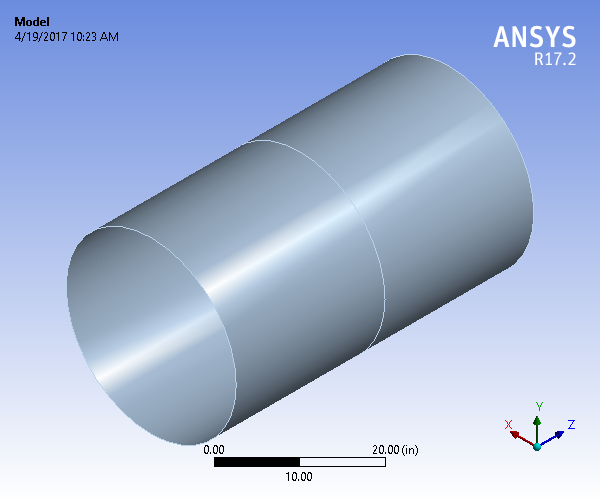
\includegraphics[scale=0.5]{4_geom}
	\caption{Geometry and coordinate system overview.}
	\label{fig:4_geom}
\end{figure}

This model utilizes a thin cylindrical surface with inwards parameterized thickness to save computational time. A series of parametric studies will be performed determine how maximum stresses vary with $t$. Note that flanges are not shown in this model as they will be added in the final run.\\

The thin surface also allows for a simple initial ANSYS generated coarse mesh (see Figure~\ref{fig:4_mesh}).

\begin{figure}[H]
	\centering
	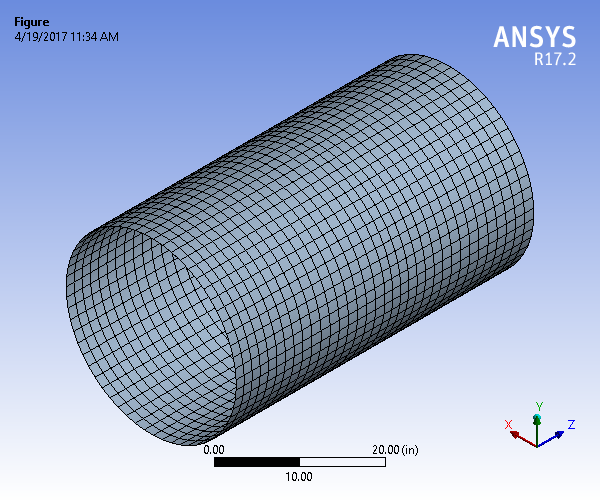
\includegraphics[scale=0.5]{4_mesh}
	\caption{Initial model coarse mesh.}
	\label{fig:4_mesh}
\end{figure}

Numerical accuracy of results will be assured by performing mesh refinement when possible in all foregoing simulations.

\section{Run 1: Uniform Pressure}
\label{section:4_R1}

The first FEA run will explore the simply uniformly loaded drum with both fixed and free ends. 

\subsection{Boundary Conditions}
\label{subsection:R1BC}

An initial simulation will be performed with fixed ends (BC as per Equation~\ref{eq:2_fixedBC}) and $t=0.500\Unit{in}$. Figure~\ref{fig:4_R1_p} shows the uniform external pressure of $1376 \Unit{psi}$ or $9.484 \Unit{MPa}$ as per \ref{eq:2_preq}.
\begin{figure}[H]
	\centering
	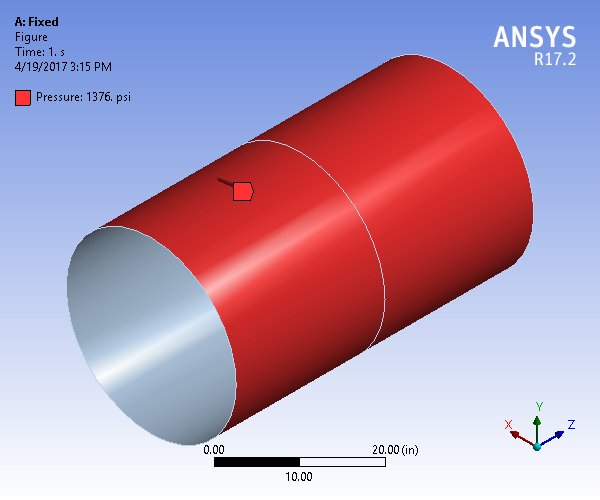
\includegraphics[scale=0.5]{4_R1_p}
	\caption{Uniform external pressure on model.}
	\label{fig:4_R1_p}
\end{figure}

\subsection{Results}

A mesh refinement is completed and yields the equivalent maximum stress results in Figure~\ref{fig:4_R1_stress} below. Note results are shown for $t=0.500\Unit{in}$.

\begin{figure}[H]
	\centering
	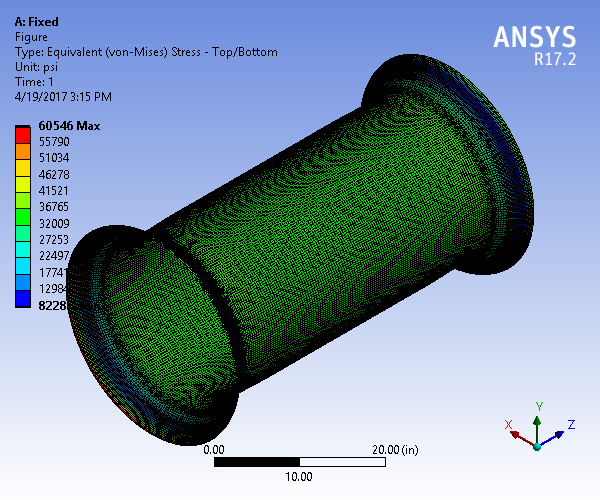
\includegraphics[scale=0.5]{4_R1_stress}
	\caption{Maximum equivalent stress results for Run 1.}
	\label{fig:4_R1_stress}
\end{figure}

It is apparent from the above figure that the fixed ends are carrying most of load. In hopes of better understanding how this uniform pressure results in stress, a parametric study will is performed by varying the drum thickness $t$ for a cylinder with both fixed and simply supported ends.


\subsection{Parametric Study}

A parametric study is perforned with a range of $t \in [0.500, 1.750]$ for both fixed and simply supported ends. The results from this simulation are shown below in Figure~\ref{fig:4_R1_sweep} \cite{EXCEL}. The allowable stress limit of $23,333 \Unit{psi}$ (Equation~\ref{eq:2_sigall}) is also shown for reference.

\begin{figure}[H]
	\centering
	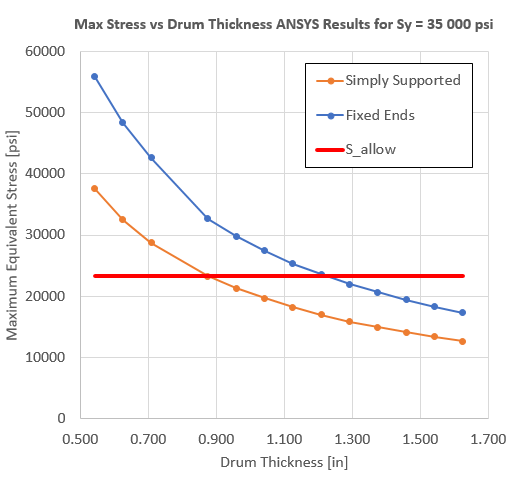
\includegraphics[scale=0.75]{4_R1_sweep}
	\caption{Results the parametric sweep for Run 1.}
	\label{fig:4_R1_sweep}
\end{figure}

From the above plot, thicknesses of $1.250 \Unit{in}$ and $0.875\Unit{in}$ are required for a uniformly loaded cylinder with fixed (Run 1A) and simply supported ends (Run 1B) respectively. These results are relatively close to their analytical counterparts. Several sources of error could be a reason for the discrepancies , those of which will be discussed in Section~\ref{subsection:5_numerr}.

\section{Run 2: Capstan Pressure}
\label{section:4_R2}
The second run elaborates on the results determined from Run 1. The aim of Run 2 is to determine how the decaying Capstan pressures translates to stress. This pressure profile represents a more realistic loading scenario.

\subsection{Boundary Conditions}

Initial results are shown for simply supported supported ends (i.e. BC as per Equation~\ref{eq:2_endBC} ) and a thickness of $0.500$ in.\\

The variable Capstan pressure is shown applied to the external surface of the cylinder in Figure~\ref{fig:4_R2_pvar}. This pressure profile is also shown in Figure~\ref{fig:4_R2_pvarplot} as per the results in Section~\ref{subsection:alt}. Note again that the pressure profile is shown for $\mu=0.05$, the worst case scenario. It is also applied beginning at the center of the drum or $z=24.5$.

\begin{figure}[H]
	\centering
	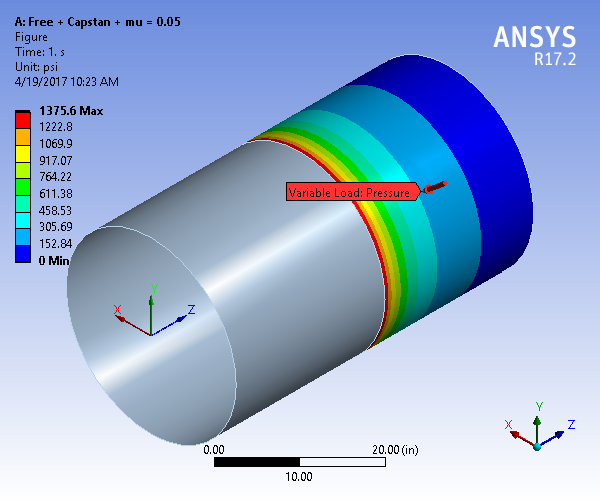
\includegraphics[scale=0.5]{4_R2_pvar}
	\caption{Variable Capstan pressure for $\mu=0.05$.}
	\label{fig:4_R2_pvar}
\end{figure}
\begin{figure}[H]
	\centering
	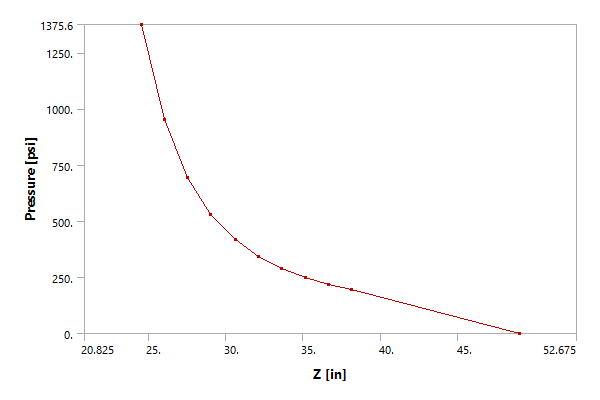
\includegraphics[scale=0.6]{4_R2_pvarplot}
	\caption{Variable Capstan pressure $p(z)$.}
	\label{fig:4_R2_pvarplot}
\end{figure}

\subsection{Results}

Total deformation results are shown below in Figure~\ref{fig:4_R2_def_mu05}. The maximum deformation seen along the $z$ axis in the $y$ direction is also shown in Figure~\ref{fig:4_R2_topdefplotmu05}.

\begin{figure}[H]
	\centering
 	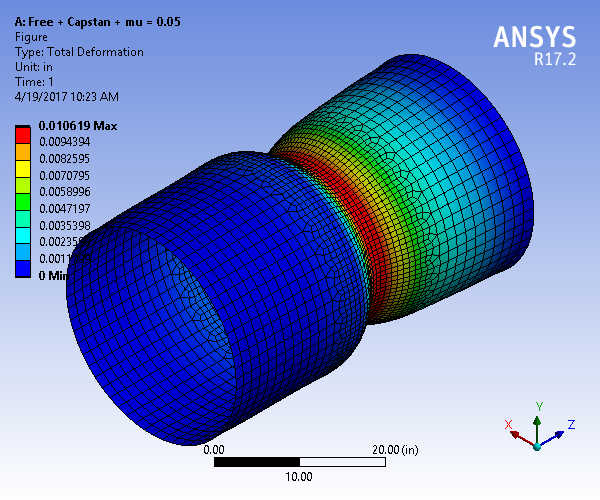
\includegraphics[scale=0.5]{4_R2_def_mu05}
 	\caption{Total deformation results for Run 2.}
 	\label{fig:4_R2_def_mu05}
 \end{figure}
 
 \begin{figure}[H]
 	\centering
 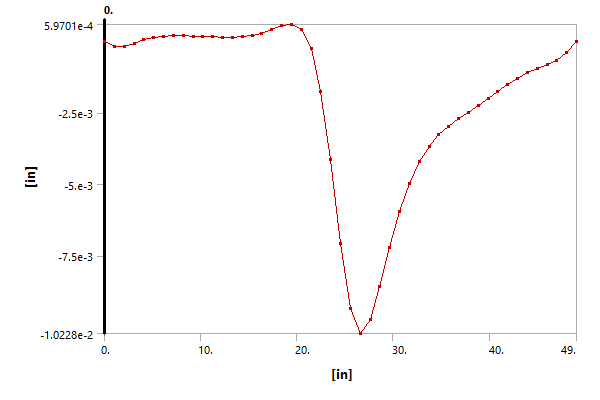
\includegraphics[scale=0.6]{4_R2_topdefplotmu05}
 	\caption{Total deformation in $y$ as a function of $z$.}
 	\label{fig:4_R2_topdefplotmu05}
 \end{figure}
 
Referring to Table~\ref{table:3_beta} for $t=0.500 \therefore \beta = 0.486 \Rightarrow x= 24.500+12.345 = 37.7$ in for $\beta x \geq 6$. From the above deformation plot, it can be observed that at $z=37.7$, deformation is nearly is zero however loading is not technically zero at this point (see Figure~\ref{fig:4_R2_pvarplot}). These observations follow those from long shell theory.\\

The maximum stress results are shown in Figure~\ref{fig:4_R2_stress_mu05} below for Run 2.

\begin{figure}[H]
	\centering
	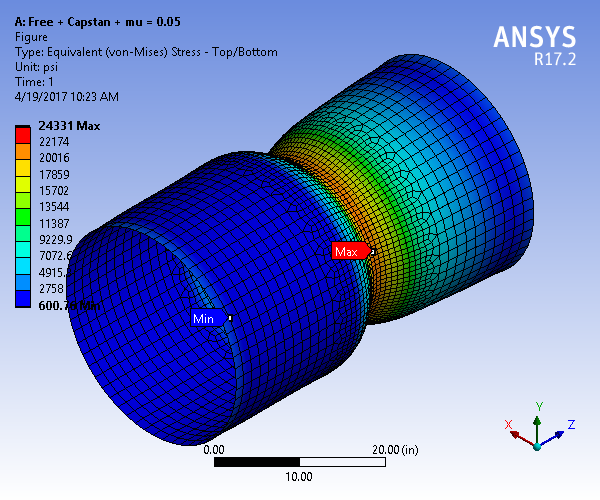
\includegraphics[scale=0.5]{4_R2_stress_mu05}
	\caption{Maximum equivalent stress results for Run 2.}
	\label{fig:4_R2_stress_mu05}
\end{figure}

Unlike the results from Run 1, it appears as though the maximum stress occurs after slightly after the location where pressure is maximum. The maximum stress is also much lower. This behavior is next explored.

\subsection{Parametric Study}

With a range of $t\in [0.15, 1.05]$, and pressure profiles for $\mu =0.05, 0.50$, maximum stress is calculated for a cylinder with both fixed and simply supported ends. The sweep results are shown below in Figure~\ref{fig:4_R2_sweep} \cite{EXCEL}.  The allowable stress limit is also shown.

\begin{figure}[H]
	\centering
	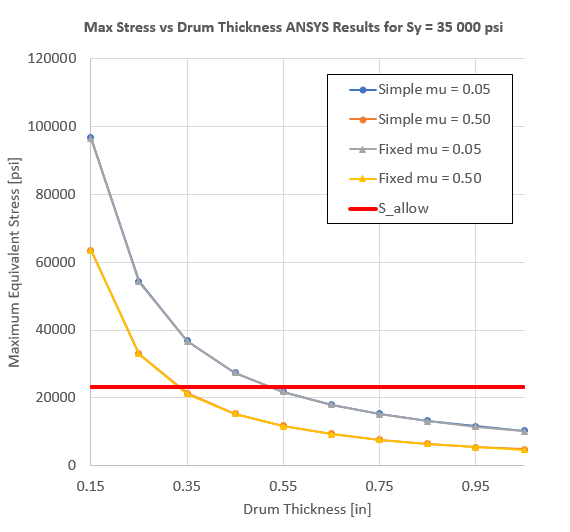
\includegraphics[scale=0.75]{4_R2_sweep_FE_SSE}
	\caption{Results of parametric study for FEA Run 2A-B.}
	\label{fig:4_R2_sweep}
\end{figure}

The main observation from the above sweep summary is that for a Capstan pressure profile beginning at the center of the drum ($z=24.5$) regardless of the end conditions. This observation can be validated through thin shell theory (i.e $\beta x \geq 6$) which dictates that internal ladings disappear once a certain distance is reached away from the location of the load application.\\

From the above plot, it appears as though a thickness of $t \geq 0.55 \Unit{in}$ would appear to be sufficient for both fixed (Run 2A) and simply supported ends (Run 2B).\\

To investigate the effects of the end conditions, the Capstan pressure was applied from $0 \leq z \leq 24.5$ (see Figure~\ref{fig:4_R2_BC_c}). The results for $t=0.500$ and $\mu=0.05$ with simply supported ends is shown in Figure~\ref{fig:4_R2_stress_c} for reference.
\begin{figure}[H]
	\centering
	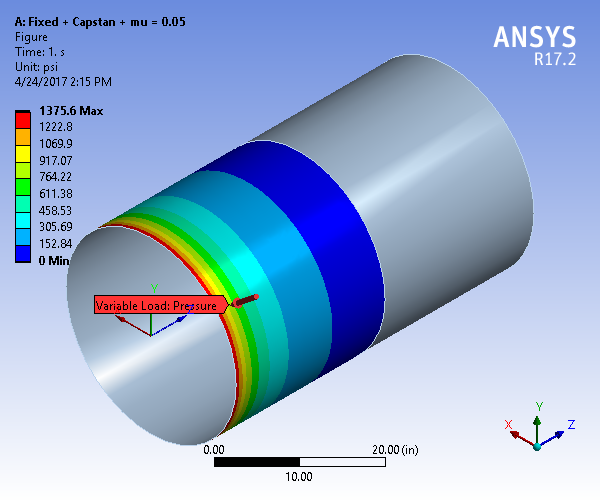
\includegraphics[scale=0.5]{4_R2_BC_c}
	\caption{Variable Capstan pressure.}
	\label{fig:4_R2_BC_c}
\end{figure}

\begin{figure}[H]
	\centering
	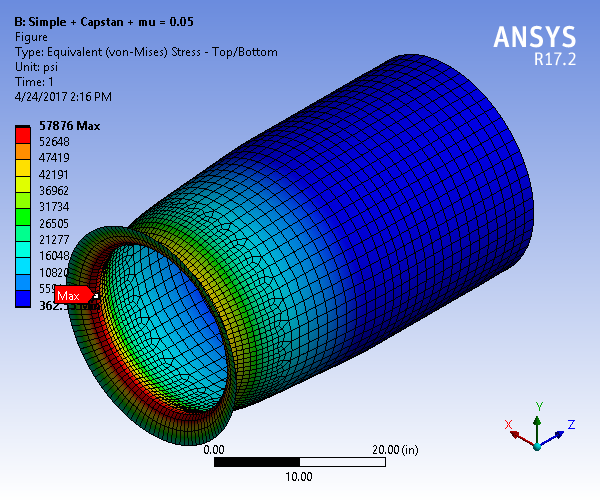
\includegraphics[scale=0.5]{4_R2_stress_c}
	\caption{Total stress results.}
	\label{fig:4_R2_stress_c}
\end{figure}

From this, a similar sweep was performed with the same aforementioned range Figure~\ref{fig:4_R2_sweep2}. With a Capstan pressure profile load applied from $0 \leq z \leq 24.5$ with $\mu=0.05$, the sweep was performed to determine the effects of the end conditions.

\begin{figure}[H]
	\centering
	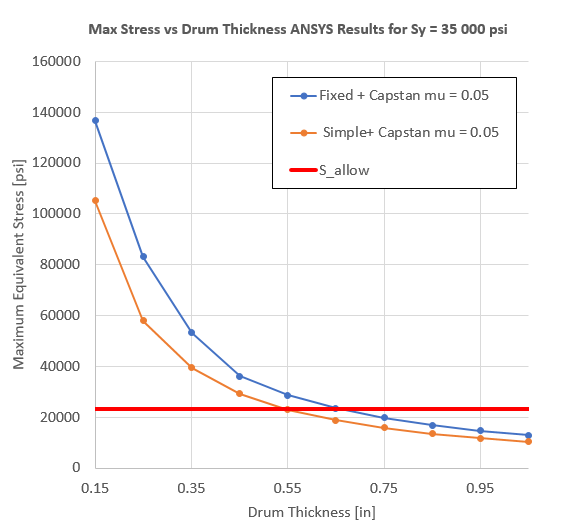
\includegraphics[scale=0.75]{4_R2_sweep_c}
	\caption{Results of parametric study for FEA Run 2C-D.}
	\label{fig:4_R2_sweep2}
\end{figure}

Moving the initial location of the pressure load application from $z=24.5$ to $z=0$ yields required thicknesses of $0.650$ and $0.550$ in for fixed (Run 2C) and simply supported ends (Run 2D), respectively.

\section{Run 3: Eigenvalue Buckling}
\label{section:4_R3}

To validate the conclusion made from Section~\ref{section:3_buckle}, Run 3 focuses on performing a linear eigenvalue buckling analysis in ANSYS. The analysis is said to be linear as in ANSYS, it is coupled with a linear static structural analysis system(see Figure~\ref{fig:4_R3_wb}).

\begin{figure}[H]
	\centering
	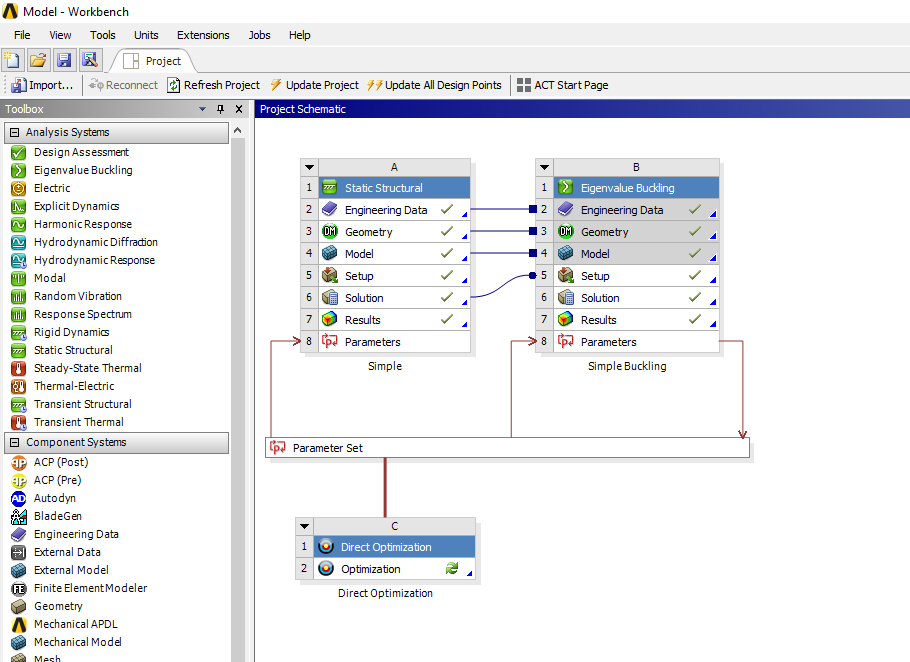
\includegraphics[scale=0.5]{4_R3_wb}
	\caption{ANSYS Workbench project schematic.}
	\label{fig:4_R3_wb}
\end{figure}

\subsection{Boundary Conditions}

ANSYS sets the linear static structural analysis system as the pre-stressed state and then peforms the eigenvalue buckling analysis. From this, load factors $\lambda$ are returned by ANSYS. These factors are defined as Equation~\ref{eq:4_loadfactor} \cite{ANSYS}.
\begin{equation}
	\label{eq:4_loadfactor}
	p' = \lambda \ p_0
\end{equation}

The critical buckling pressure $p'$ based on the pre-stressed state is simply a multiplier $\lambda$ of the applied load $p_0$. For this reason, a uniform unit load pressure of $p_0 = 1\Unit{psi}$ is applied in the coupled static structural system. Furthermore, the ends will be simply supported to match the BC from Section~\ref{section:3_buckle}.\\


With the ends simply supported (Equation~\ref{eq:2_endBC}), the unit pressure load is applied to external surface (see Figure~\ref{fig:4_R3_BC}). Also, for comparison of critical buckling calculations in Section~\ref{section:3_buckle}, a thickness of $t=0.418\Unit{in}$ is used in the foregoing results. 

\begin{figure}[H]
	\centering
	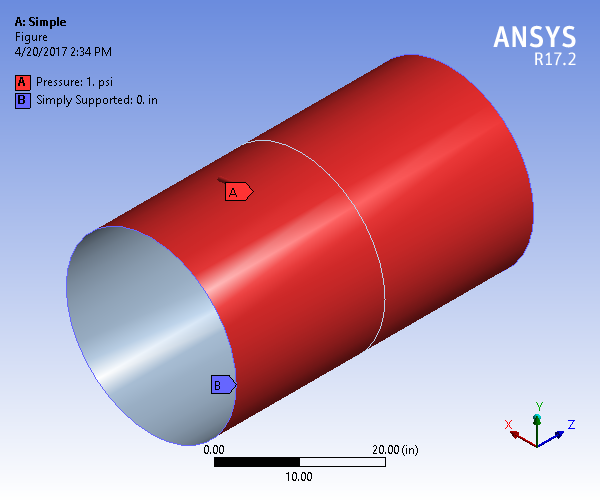
\includegraphics[scale=0.5]{4_R3_BC}
	\caption{Eigenvalue buckling analysis BC.}
	\label{fig:4_R3_BC}
\end{figure}

\subsection{Results}

Unfortunately, ANSYS is unable to perform a mesh refinement study for a coupled system analysis hence, an initial extra fine mesh is used to assure numerically accurate results on the first iteration. Results are shown below (see Figure~\ref{fig:4_R3_mode1}) for the first eigenvalue or mode $\psi = 1$.
\begin{figure}[H]
	\centering
	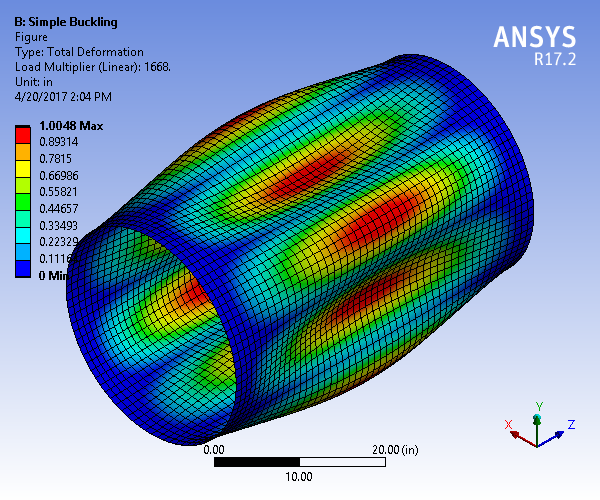
\includegraphics[scale=0.5]{4_R3_mode1}
	\caption{Total deformation results for mode $\psi = 1$.}
	\label{fig:4_R3_mode1}
\end{figure}

From above, a load factor of $\lambda = 1668$ is calculated for $t= 0.418\Unit{in}$. This value is within about $21.2\%$ of the expected analytical results of Section~\ref{section:3_buckle}, which is a reasonable margin for a first iteration. Note that the above results do not represent actual displacements but simply to visualize how the cylinder would deform when excited to the first mode \cite{ANSYS}.

\subsection{Parametric Study}

Again for $t\in [0.05, 1.05]$, a parametric study is performed. Results for the first, fifth and tenth mode (i.e. $\psi = 1, 5, 10$) are plotted against the thickness range of interest in Figure~\ref{fig:4_R3_modesweep} below, as per \cite{PYTHON} script in Appendix~\ref{appendix:a4}. The required pressure of $p =1376\Unit{psi}$ is also shown for reference.

\begin{figure}[H]
	\centering
	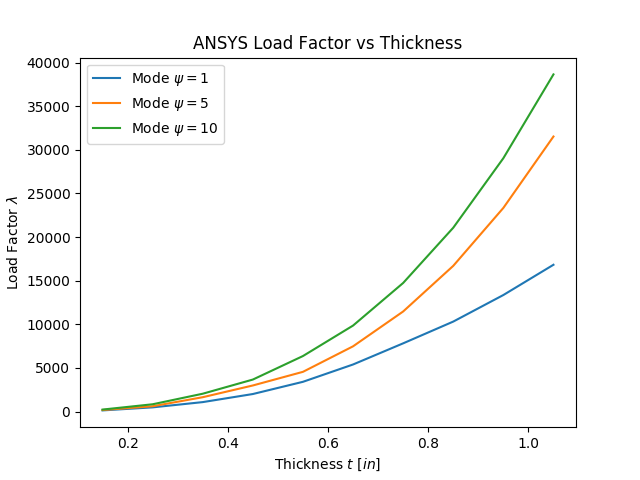
\includegraphics[scale=0.75]{4_R3_modesweep}
	\caption{Parametric sweep results for various $t, \psi$.}
	\label{fig:4_R3_modesweep}
\end{figure}

\begin{figure}[H]
	\centering
	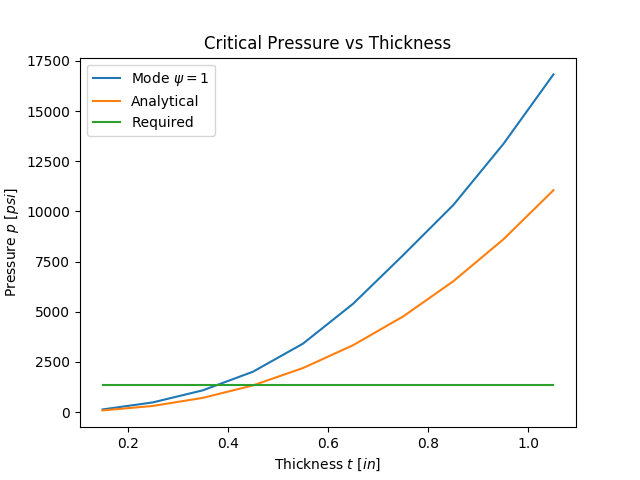
\includegraphics[scale=0.75]{4_R3_comp}
	\caption{Comparison of analytical and FEA results.}
	\label{fig:4_R3_comp}
\end{figure}

Focusing on the buckling mode of interest (i.e. $\psi=1$), observations from the above plots confirms the conclusion from Section~\ref{section:3_buckle} that failure by stress will occur before buckling. If anything, FEA results show that the analytical results previously calculated are more conservative however, this could likely be attributed to the numerical error as previously discussed.\\

The FEA Run 3 shows that to achieve a critical buckling pressure of $p'=p_{req}$, a thickness of $t=0.375\Unit{in}=9.5\Unit{mm}$ is sufficient.

\section{Run 4: Flanges}
\label{section:4_R4}
Due to time constraints, Run 4 serves as a preliminary benchmark for sizing the thickness of a 36 in OD flange. This foregoing FEA run utilizes a constant barrel $t=0.625\Unit{in}$.\\

Expanding on the thin cylindrical geometry from Figure~\ref{fig:4_geom}, circular flanges are added to each end, also modeled as thin surfaces with parameterized thickness. Figure~\ref{fig:4_R4_mesh} below shows the mesh for the modeled assembly. An initial fine mesh  is used again as convergence for numerical precision is not possible for assemblies in ANSYS.
\begin{figure}[H]
	\centering
	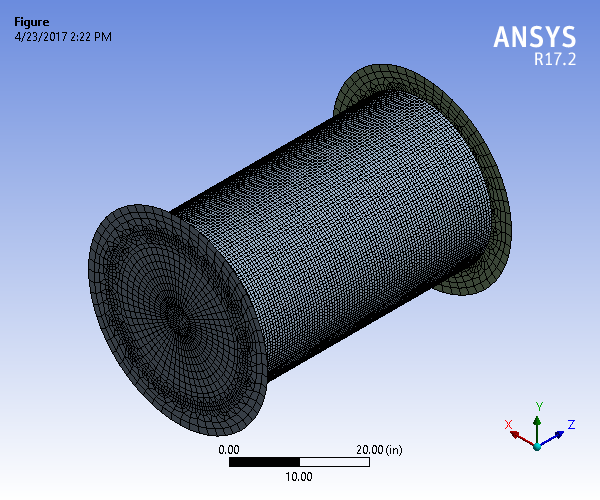
\includegraphics[scale=0.5]{4_R4_mesh}
	\caption{Drum assembly fine mesh.}
	\label{fig:4_R4_mesh}
\end{figure}

\subsection{Boundary Conditions}

The worst case flange loading is explored by applying uniform external pressure of 1376 psi. Also, the circumference of a 5 in OD circular region is held fixed to model the winch shafts (see Figure~\ref{fig:4_R4_BC}).
\begin{figure}[H]
	\centering
	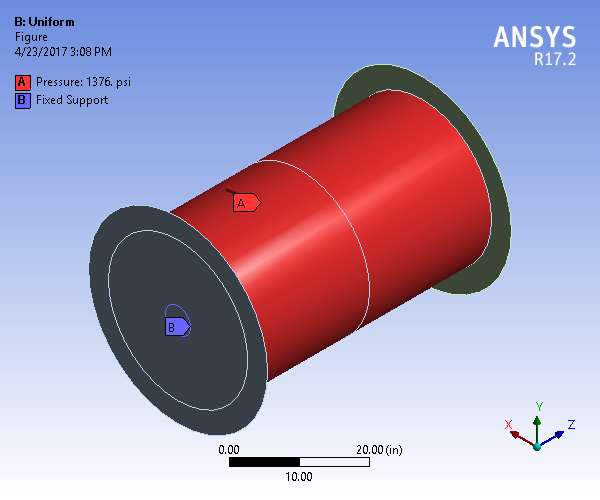
\includegraphics[scale=0.5]{4_R4_BC}
	\caption{Uniform external pressure and fixed shaft flange region.}
	\label{fig:4_R4_BC}
\end{figure}

\subsection{Results}

Both maximum stress of entire assembly (see Figure~\ref{fig:4_R4_res2}) and single flange (see Figure~\ref{fig:4_R4_res1}) are shown below. Note these results are for 0.125 in thick flanges.

\begin{figure}[H]
	\centering
	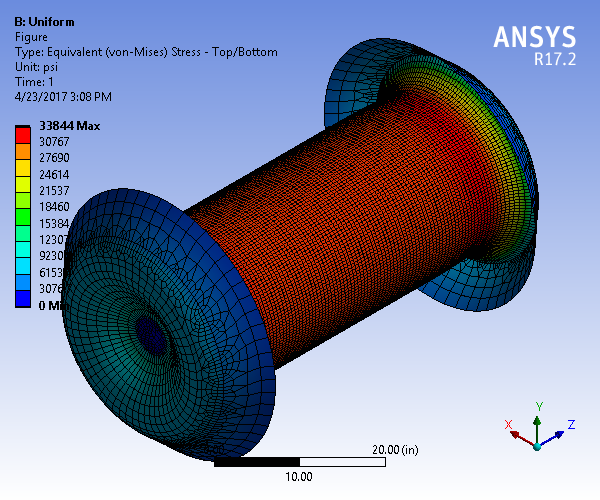
\includegraphics[scale=0.5]{4_R4_res2}
	\caption{Drum assembly stress results.}
	\label{fig:4_R4_res2}
\end{figure}
\begin{figure}[H]
	\centering
	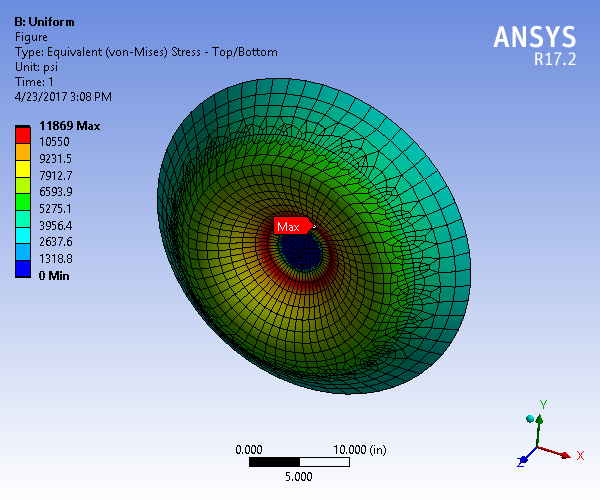
\includegraphics[scale=0.5]{4_R4_res1}
	\caption{Flange stress results for $t=0.125 \Unit{in}$.}
	\label{fig:4_R4_res1}
\end{figure}

The first observation from these above plots is that the drum barrel will experience the highest stress state.\\

Next, based on the stress results shown for the shaft side of the flange, maximum stress is exhibited near the perimeter of the 5 in OD fixed circular region. It must be noted however that even for a relatively thin flange (0.125 in) the maximum stress is still reaches about half ($\approx 50.8\%$) of the allowable limit.

\subsection{Parametric Study}

The final parametric study of this section explores flanges thicknesses $\in [0.063, 1.000]$. A second model utilizing the worst case Capstan pressure profile ($\mu=0.05$) instead of the uniform 1376 psi. The results are shown below in Figure~\ref{fig:4_R4_sweep} \cite{EXCEL}.

\begin{figure}[H]
	\centering
	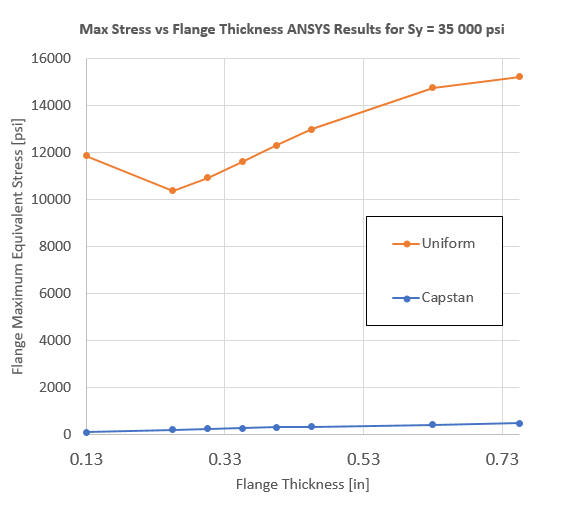
\includegraphics[scale=0.75]{4_R4_sweep}
	\caption{Results of parametric study for FEA Run 4.}
	\label{fig:4_R4_sweep}
\end{figure}

At first glance, the above sweep results do not appear to be relevant however after much discussion with both John Umina and Ephraim Lanford, some sense can be made. Focusing on the uniform pressure results would appear that a thickness of $t\approx$ 0.250 in / 6.4 mm  is the optimal candidate. The reason for the increase in flange stress with thickness could be a result of the effects of the fixed end.\\

As for the Capstan sweep results, the low maximum stress values raise the question of the simulation's validity. Again due to time constraints, these results will not be refined however, should be investigated in the future.

